\let\negmedspace\undefined
\let\negthickspace\undefined
\documentclass[journal]{IEEEtran}
\usepackage[a5paper, margin=10mm, onecolumn]{geometry}
\usepackage{lmodern} % Ensure lmodern is loaded for pdflatex
\usepackage{tfrupee} % Include tfrupee package

\setlength{\headheight}{1cm} % Set the height of the header box
\setlength{\headsep}{0mm}     % Set the distance between the header box and the top of the text

\usepackage{gvv-book}
\usepackage{gvv}
\usepackage{cite}
\usepackage{amsmath,amssymb,amsfonts,amsthm}
\usepackage{algorithmic}
\usepackage{graphicx}
\usepackage{textcomp}
\usepackage{xcolor}
\usepackage{txfonts}
\usepackage{listings}
\usepackage{enumitem}
\usepackage{mathtools}
\usepackage{gensymb}
\usepackage{comment}
\usepackage[breaklinks=true]{hyperref}
\usepackage{tikz}
\usepackage{tkz-euclide} 
\usepackage{listings}
\def\inputGnumericTable{}                                 
\usepackage[latin1]{inputenc}                                
\usepackage{color}                                            
\usepackage{array}                                            
\usepackage{longtable}                                       
\usepackage{calc}                                             
\usepackage{multirow}                                         
\usepackage{hhline}                                           
\usepackage{ifthen}                                           
\usepackage{lscape}
\usepackage{listings}
\usetikzlibrary{matrix}

\begin{document}

\bibliographystyle{IEEEtran}
\vspace{3cm}

\title{10.3.3.1.5}
\author{EE24BTECH11003 - Akshara Sarma Chennubhatla}
% \maketitle
% \newpage
% \bigskip
{\let\newpage\relax\maketitle}

\renewcommand{\thefigure}{\theenumi}
\renewcommand{\thetable}{\theenumi}
\setlength{\intextsep}{10pt} % Space between text and floats

\textbf{Question:}
\newline
Solve the following pair of linear equations,
\begin{align}
	\sqrt{2}x + \sqrt{3}y &= 0\\
	\sqrt{3}x - \sqrt{8}y &= 0
\end{align}
\textbf{Solution:\\}
Let
\begin{align}
	\vec{x} = \myvec{x\\y}
\end{align}
Expressing the system in matrix form,
\begin{align}
	\myvec{\sqrt{2} & \sqrt{3} \\ \sqrt{3} & -\sqrt{8}}\vec{x} &= \myvec{0 \\ 0}\\
	\text{which is of the form } A\vec{x} &= \vec{0}
\end{align}
Any non-singular matrix $A$ can be expressed as a product of an upper triangular matrix $U$ and a lower triangular matrix $L$, such that
\begin{align}
	A &= LU\\
	\implies LU\vec{x} &= \vec{0}
\end{align}
$U$ is determined by row reducing $A$ using a pivot,
\begin{align}
	\myvec{\sqrt{2} & \sqrt{3}\\\sqrt{3} & -\sqrt{8}} \xrightarrow {R_2 \to R_2 - \sqrt{\frac{3}{2}}R_1} \myvec{\sqrt{2} & \sqrt{3}\\0 & -\sqrt{8} - \frac{3}{2}}
\end{align}
Let 
\begin{align}
	L = \myvec{1 & 0\\l & 1}
\end{align}
$l$ is the multiplier used to zero out $a_{21}$ in $A$.
\begin{align}
	L = \myvec{1 & 0 \\ \sqrt{\frac{3}{2}} & 1}
\end{align}
This $LU$ decomposition could also be computationally found using Doolittle's algorithm. The update equation is given by,
\begin{align}
	U_{ij} &= \begin{cases}
		A_{ij} & \quad i = 0\\
		A_{ij} - \sum_{k = 0}^{i - 1} L_{ik} U_{kj} & \quad i > 0
	\end{cases}\\
	L_{ij} &= \begin{cases}
		\frac{A_{ij}}{U_{jj}} & \quad j = 0, U_{jj} \neq 0\\
		\frac{A_{ij} - \sum_{k = 0}^{j - 1} L_{ik} U_{kj}}{U_{jj}} & \quad j > 0
	\end{cases}\\
\end{align}
\newline
Let $\vec{y} = U\vec{x}$,
\begin{align}
	L\vec{y} = \vec{0} \label{y_eq}
\end{align}
After we find $\vec{y}$, we find $\vec{x}$ using the following equation,
\begin{align}
	U\vec{x} = \vec{y} \label{x_eq}
\end{align}
Applying forward substitution on equation $\brak{\ref{y_eq}}$, we get,
\begin{align}
	\myvec{1 & 0\\\sqrt{\frac{3}{2}} & 1}\myvec{y_1\\y_2} &= \myvec{0\\0}\\
	y_1 &= 0\\
	\sqrt{\frac{3}{2}}y_1 + y_2 &= 0\\
	\implies \myvec{y_1\\y_2} &= \myvec{0\\0}
\end{align}
Substituting $\vec{y}$ in equation $\brak{\ref{x_eq}}$, we get,
\begin{align}
	\myvec{\sqrt{2} & \sqrt{3}\\0 & -\sqrt{8} - \frac{3}{2}} \myvec{x\\y} &= \myvec{0\\0}\\
	\sqrt{2}x + \sqrt{3}y &= 0\\
	\brak{-\sqrt{8} - \frac{3}{2}}y &= 0\\
	\implies x &= 0, y = 0\\
	\implies \myvec{x\\y} &= \myvec{0\\0}
\end{align}
This shows that the pair of linear equations have exactly one solution.
\newpage
Below is the $LU$ decomposition of this matrix got through the c code.

\begin{lstlisting}
L:
1.000000  0.000000 
1.224745  1.000000 

U:
1.414214  1.732051 
0.000000  -4.949748	
\end{lstlisting}

Below is the plot of the pair of lines representing the linear equations and their point of intersection.
\begin{figure}[h!]
	\centering
	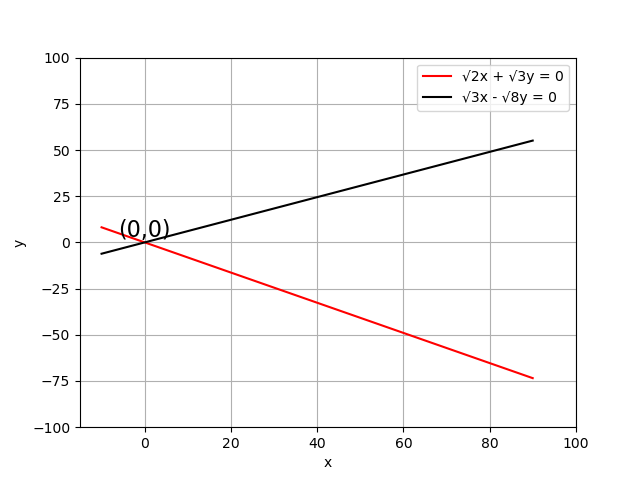
\includegraphics[width=1\columnwidth]{figs/simulated.png}
	\caption{Plot of the linear equations and their intersection point}
	\label{label}
\end{figure}
\end{document}
